\chapter{Casebeskrivelser}
\label{kap:casebeskrivelser}
I dette kapittelet gir vi en detaljert beskrivelse av hvert case som gjennomføres. 

\section{Case 1: Ulovlig fildeling på universitetsnettet}
\label{sec:case_fildeling}
NTNU har ansvar for nettet hos studenthyblene studentene leier fra Sit. Når studenter driver med ulovlig fildeling fra hybelen vil NTNU kunne holdes ansvarlig. Dette er et problem for NTNU, ikke bare i form av skadet omdømme, men det kan også være problematisk hvis opphavsrettshaverne går juridisk til verks. Oppgaven i dette caset er derfor å finne, ved hjelp av rotårsaksanalysemetodikken, rotårsaken(e) til hvorfor studenter laster ned opphavsrettsbeskyttet materiale. Det skal også presenteres en tydelig tiltaksplan for å eliminere rotårsaken(e).

\subsubsection{Oversikt over oppgaven}
Advokater til diverse filmselskaper ser etter IP-adresser til personer som laster ned opphavsrettsbeskyttede materiale, og sender disse personene notifikasjoner på e-post. Hver måned får NTNU ca. 150 og 200 unike notifikasjoner om brudd på opphavsretten ved ulovlig fildeling. Vi kan se at dette nummeret går kraftig ned i sommermånedene, som kan tilsi at studentene er hovedgrunnen til bruddene på opphavsrett. Disse tallene kan vi se i figur \ref{fig:copyright} under.

\begin{figure}[H]
    \centering
    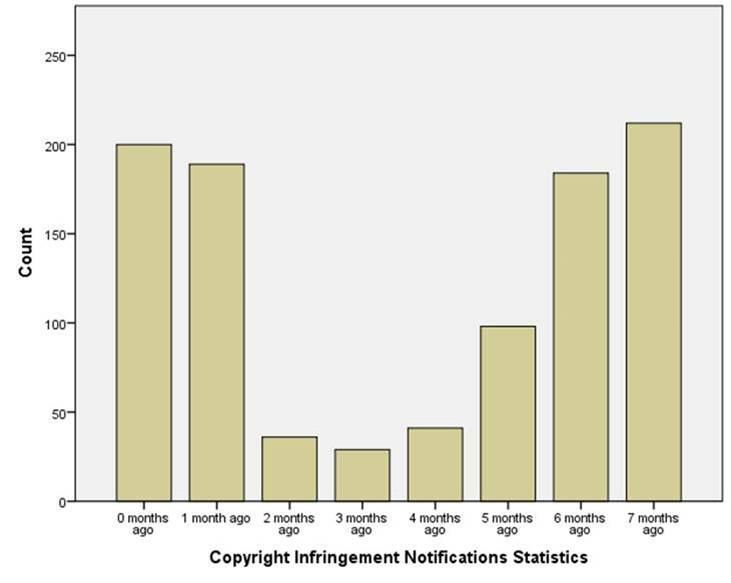
\includegraphics[scale=0.8]{case_1/bilder/copyright.jpg}
    \caption[Copyright Infringement Notifications]{Oversikt over antall notifikasjoner i sommerhalvåret}
    \label{fig:copyright}
\end{figure}

Dersom opphavsrettshaverne begynner å håndheve opphavsretten i brevene de sender, kan NTNU komme i en dårlig posisjon. I dag gjør ikke NTNU noe med de mange brevene de får, grunnet de store mengdene og at det er en fulltidsjobb i seg selv å håndtere dem.

Ulovlig fildeling foregår som regel ved hjelp av en protokoll som heter BitTorrent, som bruker peer-to-peer teknologi. Universitetet har per dags dato ikke mulighet til å blokkere denne, da protokollen også innebærer legitimt bruk. NTNU kan heller ikke overvåke de som laster ned ulovlig, og sperre nettet til disse \footnote{Informasjon fra oppdragsgiver}.

I caset avgrenser vi oss til NTNU Gjøvik, og ser bare på nettverket til de ulike studentbyene tilknyttet Sit Bolig. Nettet på campus faller ikke under problemstillingen, da universitetet kan overvåke dette.